\newfontfamily\BBSevenIPA[Path=vendor/fonts/,BoldFont=CharisSIL-Bold.ttf,ItalicFont=CharisSIL-Italic.ttf,BoldItalicFont=CharisSIL-BoldItalic.ttf]{CharisSIL-Regular.ttf}
\newcommand{\bipa}[1]{{\BBSevenIPA #1}}
\chapter{LA PHONÉTIQUE ARTICULATOIRE}
\label{chapter-7}
\markright{La phonétique articulatoire}
\origpage{203}{189}
\begin{keybox}[Plan du chapitre]
\small
\textbf{I.\quad PRÉSENTATION DE L’APPAREIL PHONATOIRE}
\begin{enumerate}[label=\arabic*.]
\item Les cavités sous-glottiques
\begin{enumerate}[label=\textcircled{\scriptsize\arabic*}]
\item Les poumons
\item Le diaphragme
\end{enumerate}
\item Le larynx, instrument à corde et à vent
\begin{enumerate}[label=\textcircled{\scriptsize\arabic*}]
\item Description du larynx
\item Les cordes vocales
\item Les différents modes phonatoires
\begin{enumerate}[label=\arabic*.]
\item Le mode écarté
\item Le mode vibratoire
\end{enumerate}
\end{enumerate}
\item Les cavités supra-glottiques
\begin{enumerate}[label=\textcircled{\scriptsize\arabic*}]
\item La cavité pharyngale
\item La cavité buccale
\item La cavité labiale
\item La cavité nasale
\end{enumerate}
\end{enumerate}
\textbf{II.\quad PRODUCTION DES CONSONNES FRANÇAISES}
\begin{enumerate}[label=\arabic*.]
\item Point et mode d’articulation
\begin{enumerate}[label=\textcircled{\scriptsize\arabic*}]
\item Le point d’articulation
\begin{enumerate}[label=\arabic*.]
\item Les lieux d’articulation
\item Les articulateurs
\end{enumerate}
\item Le mode d’articulation
\end{enumerate}
\item Classification des consonnes
\end{enumerate}
\textbf{III. LA PRODUCTION DES VOYELLES DU FRANÇAIS}
\begin{enumerate}[label=\arabic*.]
\item Le trapèze vocalique
\begin{enumerate}[label=\textcircled{\scriptsize\arabic*}]
\item Le degré d’aperture
\item Le degré d’antériorité
\item Les voyelles arrondies et non arrondies
\item Les voyelles orales et nasales
\end{enumerate}
\origpage{204}{190}
\item Classification des voyelles
\item Tableaux récapitulatifs
\end{enumerate}
\textbf{Exercices}\par
\textbf{Pour aller plus loin}\par
\textbf{Glossaire}
\end{keybox}

\origpage{205}{191}
\begin{keybox}[Introduction]
\renewcommand{\thempfootnote}{校\arabic{editorialnote}}
L’étude des sons utilisés dans le langage humain s’appelle la phonétique. Selon le point de vue adopté, la phonétique se divise en trois sous branches :
\begin{itemize}
\item la phonétique articulatoire : la plus ancienne des trois branches de la phonétique, elle étudie la manière dont les sons du langage humain sont produits.
\item la phonétique acoustique étudie la transmission des sons dans l’air selon ses caractéristiques physiques (fréquence, intensité, durée, etc.).\ednote{原文 ses caractéristiques 如此；此处所列频率、强度、时长是声音的物理特征，若回指 les sons，应为 leurs caractéristiques。}
\item la phonétique auditive étudie les processus d’audition du langage et la façon dont l’humain perçoit et reconnaît les sons.
\end{itemize}
Dans ce chapitre, nous allons nous limiter à la phonétique articulatoire, discipline qui au 19e siècle a réalisé de grands progrès grâce à l’invention d’un outil, le laryngoscope, qui permet d’examiner le larynx. L’idée originale est venue d’un professeur de chant espagnol, Manuel Garcia (1805-1906), qui souhaitait voir ses cordes vocales en pleine action lorsqu’il chantait. Un jour de l’été 1855, alors qu’il se promenait à Paris dans les jardins du Palais-Royal, c’est en voyant un rayon de soleil se réfléchir sur la poignée en argent de sa canne qu’il a eu l’idée de regarder ses cordes vocales à l’aide de deux miroirs : l’un dirigeant la lumière et l’autre lui permettant de regarder au fond de sa gorge. Rentré à Londres, où il vivait, il a rédigé un mémoire intitulé « Observations physiologiques sur la voix humaine » qu’il a présenté à la Société royale de Londres. En 1857, Ludwig Türck (1810-1868), professeur de médecine à Vienne, a eu connaissance des travaux de Garcia et a développé un prototype de laryngoscope. Leur invention a grandement contribué à percer le mystère de la voix, auquel le présent chapitre est consacré.
\end{keybox}

\section{PRÉSENTATION DE L’APPAREIL PHONATOIRE}
Après avoir établi dans le chapitre 2 que seul l’homme parle, il convient de se poser question du « comment ».\ednote{原文 se poser question 如此；应为 se poser la question。} Le processus de production de parole chez l’homme est un mécanisme très complexe, et une grande quantité d’organes et de muscles entrent dans la production de sons des langues naturelles.
\begin{center}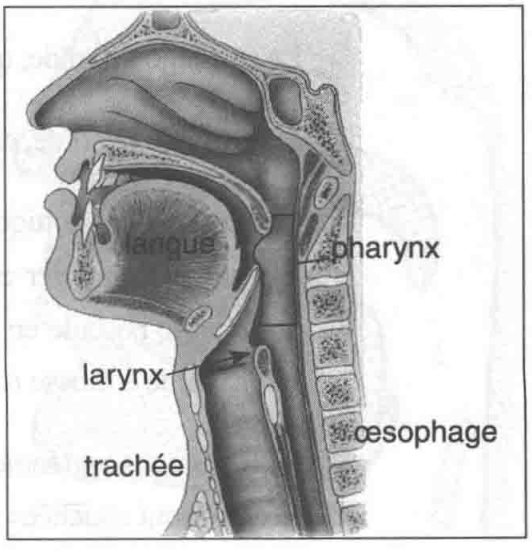
\includegraphics[width=.36\linewidth]{assets/ch07_vocal_tract.png}\end{center}

\origpage{206}{192}
\subsection{Les cavités sous-glottiques}
Le fonctionnement de l’appareil phonatoire humain repose sur l’interaction de trois grandes classes d’organes : les poumons, le larynx et les cavités supra-glottiques (la glotte désignant la partie du larynx qui comprend les deux cordes vocales). Les deux premières classes fournissent ce qui est essentiel pour la production de n’importe quel son, qu’il soit musical ou langagier : une source d’air et une source de bruit.\ednote{“n’importe quel son”范围过大。此处描述肺部气流及喉部参与的典型言语发声过程，不是所有声音的必要条件；例如本章后文也说明清擦音不依赖声带振动，且国际音标表另列非肺部气流辅音。见\ecite{41}。}
\minititle{\textcircled{\scriptsize 1}\quad Les poumons}
La fonction primordiale des poumons est évidemment de permettre au corps de s’oxygéner. Cependant, les poumons fournissent aussi une source d’air qui est utilisée pour produire des sons.
\minititle{\textcircled{\scriptsize 2}\quad Le diaphragme}
Lors de la phase d’inspiration, c’est l’action conjointe du diaphragme, qui se contracte et s’abaisse, et des muscles intercostaux qui permet de créer un vide dans les poumons qui se remplissent alors d’air. Lors de l’expiration, le diaphragme se relâche et laisse ainsi s’échapper des poumons l’air utilisé pour produire des sons.
\begin{center}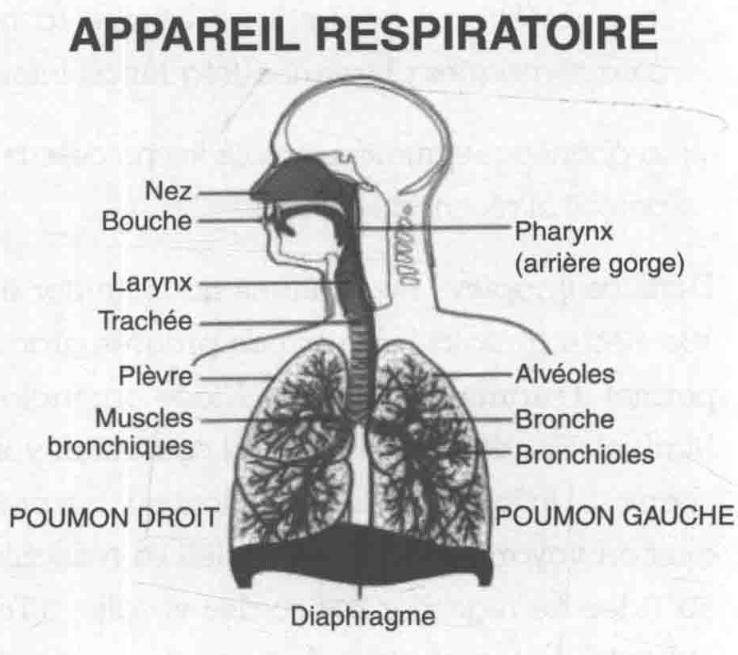
\includegraphics[width=.49\linewidth]{assets/ch07_respiratory.png}\end{center}
\subsection{Le larynx, instrument à corde et à vent}
Lorsque l’air est expulsé des poumons, il passe à travers la trachée avant d’arriver dans un tube formé de cartilages et de muscles : le larynx.
\minititle{\textcircled{\scriptsize 1}\quad Description du larynx}
Le larynx est un organe cartilagineux de l’appareil respiratoire situé au niveau de la gorge. Intermédiaire entre le pharynx et la trachée, il abrite les cordes vocales. Il contient :
\begin{itemize}
\item Le cartilage thyroïde, qui forme le relief de la « pomme d’Adam ».
\item Le cartilage cricoïde, en forme de bague, situé dans la partie inférieure du larynx.
\item Le cartilage épiglottique, en forme de cuillère. Orienté vers le haut, il permet la respiration en laissant l’air circuler entre le pharynx et le larynx. Au cours de la déglutition, son extrémité postérieure bascule en arrière et en bas, ce qui participe à l’occlusion du larynx et empêche la survenue de « fausse route », c’est-à-dire d’inhalation d’aliments.
\item Les cartilages aryténoïdes : en forme de pyramide, situés à l’arrière des cordes vocales, c’est à eux que sont attachées les cordes vocales.
\end{itemize}

\origpage{207}{193}
\minititle{\textcircled{\scriptsize 2}\quad Les cordes vocales}
Gardées ouvertes ou fermées par les cartilages aryténoïdes, les cordes vocales peuvent s’ouvrir et se refermer très rapidement : jusqu’à 400 fois par seconde chez les enfants par exemple. Leur vibration produit des variations de pression dans l’air qui sont perçues comme des sons par l’oreille humaine. Une voix typique d’homme résulte de mouvements d’ouverture de 100 à 120 fois par seconde, alors que celle d’une femme est produite par 175 à 250 vibrations des cordes vocales par seconde.
\minititle{\textcircled{\scriptsize 3}\quad Les différents modes phonatoires}
Les cordes vocales sont utilisées de plusieurs façons afin de satisfaire les besoins de la respiration et de la production des sons langagiers.
\minititle{1. Le mode écarté}
Lors de la respiration, les cordes vocales sont totalement écartées et aucun son n’est produit par ces dernières. En phonation, si vous placez votre main sur votre gorge et prononcez le son « ssssss », vous ne ressentirez aucune vibration. Les consonnes ainsi articulées sans vibration des cordes vocales sont appelées consonnes « sourdes » (ou « non voisées »).
\minititle{2. Le mode vibratoire}
Lorsque les cordes vocales s’écartent et se rapprochent très rapidement de façon à interrompre le flot d’air qui passe entre elles, on parle de mode vibratoire. Les vibrations ainsi produites vont produire des consonnes « sonores » (ou « voisées »). Placez votre main sur votre gorge et prononcez « zzzzzz » (voisé) : les vibrations perçus par votre main indiquent que ce sont voisé.\ednote{原文 perçus、ce sont voisé 如此；分别应为 perçues 和 ce son est voisé，句意为所感到的振动表明这个音有声。}
\subsection{Les cavités supra-glottiques}
Les cavités supra-glottiques renferment les organes permettant de modifier le son émis par le travail conjoint des poumons, du larynx et des cordes vocales. Le bruit émis par les cordes vocales ressemble à un ballon qui se dégonfle. En sortant de la glotte, les résonateurs vont l’amplifier, et les organes vocaux supérieurs vont le transformer en voyelles et en consonnes.
\minititle{\textcircled{\scriptsize 1}\quad La cavité pharyngale}
Cette cavité ne joue aucun rôle en français,\ednote{“在法语中不起任何作用”过强，也与上一段把声门上腔体作为共鸣腔的说明不一致。不能把“不以独立咽辅音为特征”与“咽腔不参与语音产生”混为一谈；咽腔在解剖上仍属喉以上的声道。咽、喉的位置见\ecite{43}。} mais dans certaines langues, comme l’arabe ou l’espagnol, l’allemand ou le chinois, elle est utilisée pour la production de certaines consonnes dites « gutturales » (du latin \textit{guttur} « gorge »).\ednote{gutturales 是宽泛的传统称呼，不等同于现代发音部位分类中的 pharyngales。国际音标表分别列软腭、小舌、咽和声门等部位；不能由“喉音”这一名称直接推断列举的辅音均在咽部形成阻碍。见\ecite{41}。}
\begin{center}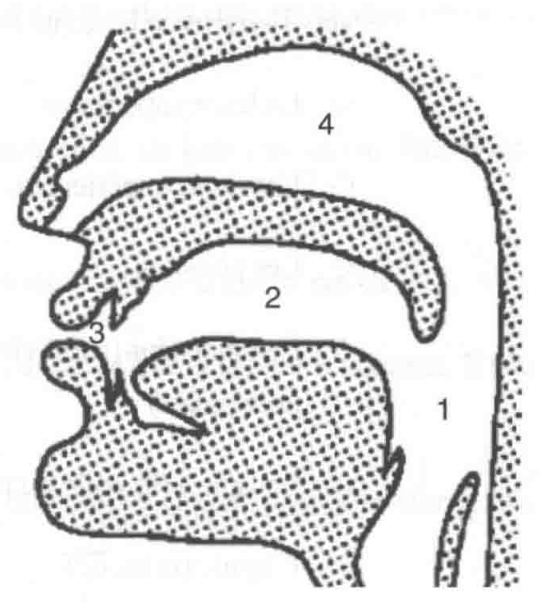
\includegraphics[width=.36\linewidth]{assets/ch07_cavities.png}\end{center}
\minititle{\textcircled{\scriptsize 2}\quad La cavité buccale}
Lorsque la luette (appelée aussi « uvule ») est collée à la cavité pharyngale, le son provenant de la glotte est complètement dirigé vers la cavité buccale.\ednote{控制口鼻通路的主要结构应表述为软腭／腭帆及腭咽闭合机制，不是单独“小舌黏在咽腔上”。小舌是软腭后缘的悬垂部分；小舌与整个软腭不能等同。下文相同的简化说法亦应据此理解。解剖区分见\ecite{42}、\ecite{43}。} L’utilisation\origcont{208}{194}de cette cavité donne lieu à des articulations orales. La forme de cette cavité peut ensuite être modifiée, et donner lieu à des consonnes et voyelles différentes, comme nous le verrons plus bas.
\minititle{\textcircled{\scriptsize 3}\quad La cavité labiale}
La cavité labiale comprend la lèvre supérieure et inférieure. Certaines articulations sont produites en utilisant le changement de forme des lèvres qui peuvent s’étirer ou s’arrondir.
\minititle{\textcircled{\scriptsize 4}\quad La cavité nasale}
Lorsque la luette est décollée de la paroi pharyngale, l’air peut entrer dans la cavité nasale, créant ainsi une articulation nasale.

Lorsque les résonateurs ont joué leur rôle de caisse de résonance, il reste alors à produire les sons de la parole : les « phones ». Commençons par les consonnes.

\section{LA PRODUCTION DES CONSONNES FRANÇAISES}
Les consonnes du français comme de la plupart des langues naturelles sont produits en utilisant les organes de la cavité buccale et les lèvres.\ednote{原文 produits 如此；与阴性复数 consonnes 一致时应为 produites。} Ces articulations peuvent être décrites selon leur mode et leur point d’articulation.
\subsection{Point et mode d’articulation}
Les modes articulatoires et les lieux d’articulation sont définis d’après les organes articulatoires utilisés dans la production des consonnes.
\minititle{\textcircled{\scriptsize 1}\quad Le point d’articulation}
Le point d’articulation est l’endroit où se trouve, dans la cavité buccale, un obstacle au passage de l’air. On distingue deux points distincts pour cette obstruction. Au niveau supérieur, il y a les lieux d’articulation contre lesquels l’air glisse pendant (obstruction partielle) ou après (obstruction totale) l’articulation. Au niveau inférieur se trouvent les articulateurs, appelés aussi organes articulatoires.
\minititle{1. Les lieux d’articulation}
Ces lieux peuvent être, en allant de l’avant vers l’arrière de la cavité buccale :
\begin{itemize}
\item La lèvre supérieure
\item Les dents supérieures
\item Les alvéoles
\item Le palais dur (subdivisé en pré-, médio- et post-palais)
\item Le \textit{vélum} (le voile du palais)
\item L’uvule (la luette)
\end{itemize}
\begin{center}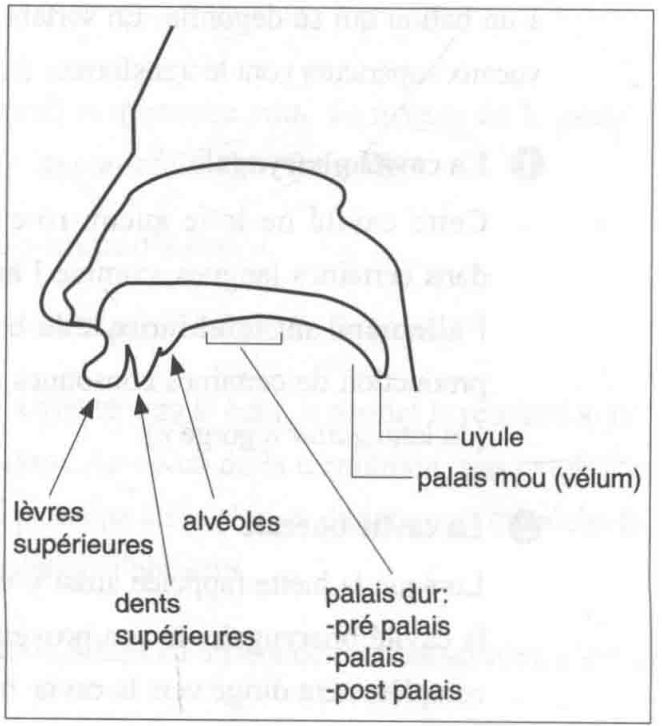
\includegraphics[width=.43\linewidth]{assets/ch07_places.png}\end{center}

\origpage{209}{195}
À chacun de ces lieux d’articulation correspond un adjectif spécifique permettant de décrire une consonne : dentale, alvéolaire, palatale, vélaire, et uvulaire. Par exemple, le \bipa{[k]} est une consonne vélaire, puisque son lieu d’articulation est le voile du palais. À ces lieux d’articulation doit s’ajouter un articulateur, qui correspond à l’un des sept organes de la partie inférieure de la cavité buccale.
\minititle{2. Les articulateurs}
Les sept articulateurs utilisables dans la production de consonnes sont :
\begin{itemize}
\item La lèvre inférieure
\item Les dents
\item L’\textit{apex} (la pointe) de la langue
\item Le pré-dos de la langue
\item Le dos de la langue
\item Le post-dos de la langue
\item La racine de la langue
\end{itemize}
\begin{center}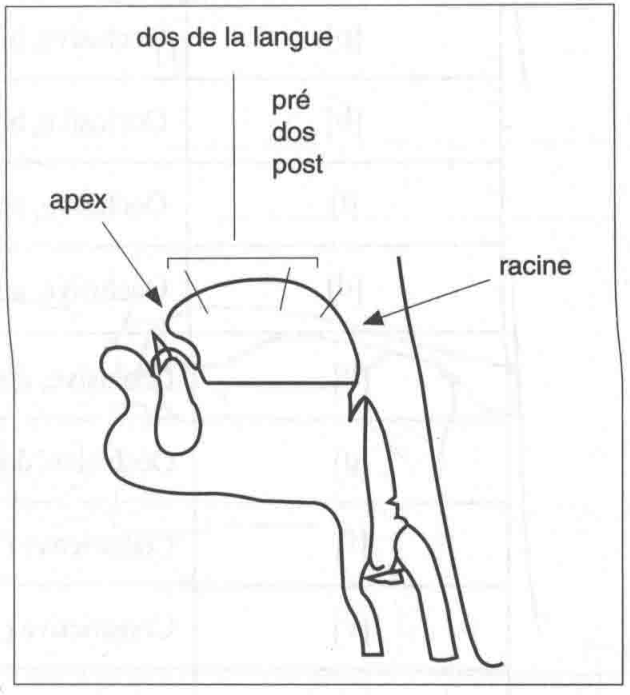
\includegraphics[width=.40\linewidth]{assets/ch07_articulators.png}\end{center}
La consonne \bipa{[p]} est bilabiale, puisque produite avec les lèvres inférieure et supérieure. De même, le \bipa{[k]} décrit plus haut est dorso-vélaire car produit avec le dos de la langue (articulateur) et le \textit{velum} (lieu d’articulation), comme ci-dessous :
\begin{center}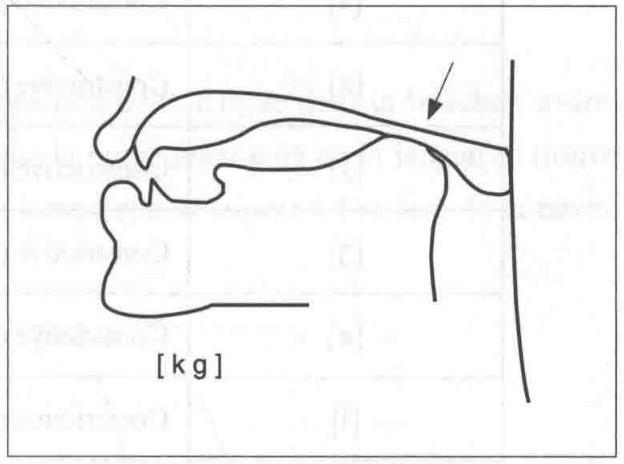
\includegraphics[width=.40\linewidth]{assets/ch07_dorsovelar.png}\end{center}
\minititle{\textcircled{\scriptsize 2}\quad Le mode d’articulation}
Une autre différence importante dans la production des consonnes en français concerne la façon dont l’air est expulsé pendant la phonation. Voici les modes articulatoires du français :
\begin{itemize}
\item Les consonnes occlusives sont des articulations qui comportent une fermeture totale et momentanée du canal vocal.
\item Les consonnes constrictives comportent un barrage partiel lors de leur réalisation. Elles sont aussi appelées « fricatives ».
\item Les consonnes nasales sont des articulations produites avec l’aide de la cavité nasale.
\item Les consonnes latérales sont produites avec le dos de la langue relevé et les bords abaissés. Il n’y a qu’une seule consonne latérale en français : le \bipa{/l/}.\ednote{对法语 \bipa{[l]}，要点是舌尖／舌端在齿龈处形成中央阻碍，气流经一侧或两侧逸出；不能仅用“舌背抬高”界定。国际音标将 \bipa{[l]} 列为齿龈边近音。见\ecite{41}。}
\item Les consonnes vibrantes sont articulées avec la langue ou la luette et produisant des vibrations.\ednote{原文 et produisant 如此；并列谓语应为 et produisent，或改写为 avec la langue ou la luette produisant des vibrations。}
\origcont{210}{196}Il n’y a qu’une seule consonne vibrante en français : le \bipa{[ʁ]}.\ednote{原文用 \bipa{[ʁ]} 表示 vibrante。国际音标中 \bipa{[ʁ]} 是浊小舌擦音，小舌颤音符号为 \bipa{[ʀ]}；字形及发音方式不可混同。此处与下表保留底本的 \bipa{[ʁ]}，不静默改成 \bipa{[ʀ]}。见\ecite{41}。}
\end{itemize}
\subsection{Classification des consonnes}
Nous pouvons décrire les consonnes du français à l’aide des quatre traits articulatoires présentés plus haut : le mode d’articulation, le point d’articulation, le mode vibratoire, et la nasalité (ou l’oralité).
\begingroup\renewcommand{\thefootnote}{校\arabic{editorialnote}}\small\renewcommand{\arraystretch}{1.22}
\begin{longtable}{|>{\centering\arraybackslash}p{.12\linewidth}|p{.79\linewidth}|}
\hline
\bipa{[p]} & Occlusive, bilabiale, sourde, orale\\\hline
\bipa{[b]} & Occlusive, bilabiale, sonore, orale\\\hline
\bipa{[t]} & Occlusive, apico-alvéodentale, sourde, orale\\\hline
\bipa{[d]} & Occlusive, apico-alvéodentale, sonore, orale\\\hline
\bipa{[k]} & Occlusive, dorso-vélaire, sourde, orale\\\hline
\bipa{[g]} & Occlusive, dorso-vélaire, sonore, orale\\\hline
\bipa{[f]} & Constrictive (fricative), labio-dentale, sourde, orale\\\hline
\bipa{[v]} & Constrictive (fricative), labio-dentale, sonore, orale\\\hline
\bipa{[s]} & Constrictive (fricative), apico-alvéolaire, sourde, orale\\\hline
\bipa{[z]} & Constrictive (fricative), apico-alvéolaire, sonore, orale\\\hline
\bipa{[ʃ]} & Constrictive (fricative), prédorso-prépalatale, sourde, orale\\\hline
\bipa{[ʒ]} & Constrictive (fricative), prédorso-prépalatale, sonore, orale\\\hline
\bipa{[ʁ]} & Constrictive (vibrante), dorso-uvulaire, sonore, orale\\\hline
\bipa{[l]} & Constrictive (sagittale), apico-alvéolaire, sonore, orale\ednote{原表把 \bipa{[l]} 记为 sagittale；与上一页的 latérale 相冲突，应为 latérale。在现代 IPA 方式分类中，\bipa{[l]} 属 lateral approximant，而非中央气流擦音。见\ecite{41}。}\\\hline
\bipa{[m]} & Occlusive, bilabiale, sonore, nasale\\\hline
\bipa{[n]} & Occlusive, apico-dentale, sonore, nasale\\\hline
\bipa{[ɲ]} & Occlusive, dorso-palatale, sonore, nasale\\\hline
\bipa{[ŋ]} & Occlusive, dorso-vélaire, sonore, nasale\\\hline
\end{longtable}\endgroup

\section{LA PRODUCTION DES VOYELLES DU FRANÇAIS}
La production des voyelles est relativement différente de celle des consonnes. Contrairement aux consonnes, elle ne nécessite pas la production de bruit de friction ou d’explosion : les voyelles sont produites avec un écoulement nettement plus libre de l’air à travers l’appareil phonatoire. Les voyelles du français sont habituellement représentées par une figure géométrique : le trapèze vocalique.

\origpage{211}{197}
\subsection{Le trapèze vocalique}
Ce trapèze, représenté sur deux dimensions, contient deux axes dont chacun renferme un type de donnée :
\minititle{\textcircled{\scriptsize 1}\quad Le degré d’aperture}
L’axe vertical du trapèze vocalique indique l’aperture, c’est-à-dire le degré d’ouverture de la bouche. Le français comprend quatre classes de voyelles divisées selon leur aperture :
\begin{itemize}
\item fermées, comme dans le mot « riz »
\item mi-fermées, comme dans le mot « ré »
\item mi-ouvertes, comme dans le mot « raie »
\item ouvertes comme dans le mot « rat »
\end{itemize}
Les deux degrés d’aperture extrêmes (fermé et ouvert) sont illustrés dans les schémas ci-dessous :
\begin{center}
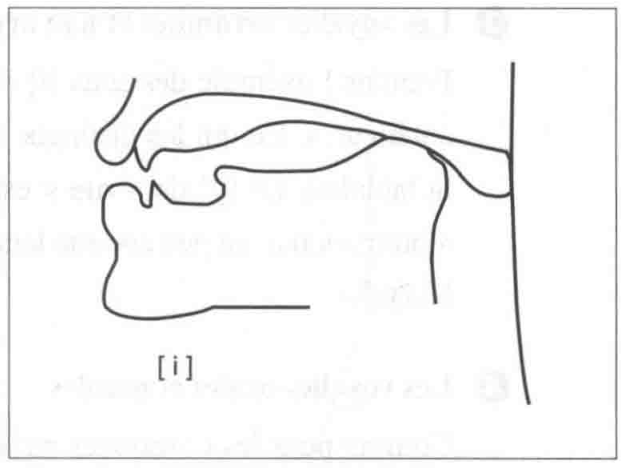
\includegraphics[width=.40\linewidth]{assets/ch07_vowel_i.png}\hfill
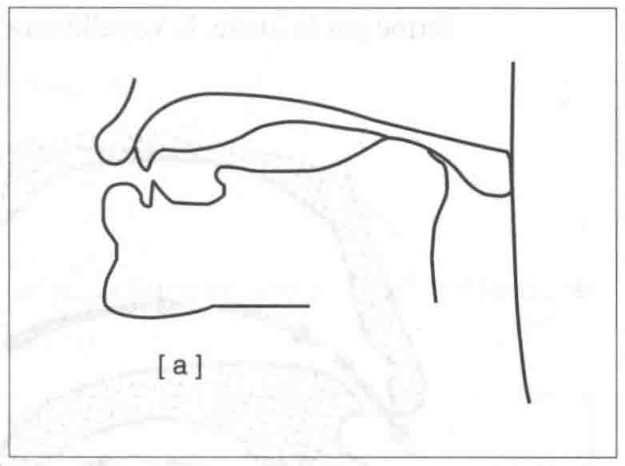
\includegraphics[width=.40\linewidth]{assets/ch07_vowel_a.png}
\end{center}
\minititle{\textcircled{\scriptsize 2}\quad Le degré d’antériorité}
L’axe horizontal du trapèze vocalique indique la position de la langue dans la bouche : avant, centre, arrière. Une voyelle est dite antérieure lorsque la partie antérieure de la langue se trouve à l’avant de la cavité buccale. Elle est postérieure lorsqu’elle se trouve à l’arrière de la cavité buccale, comme ci-dessous :
\begin{center}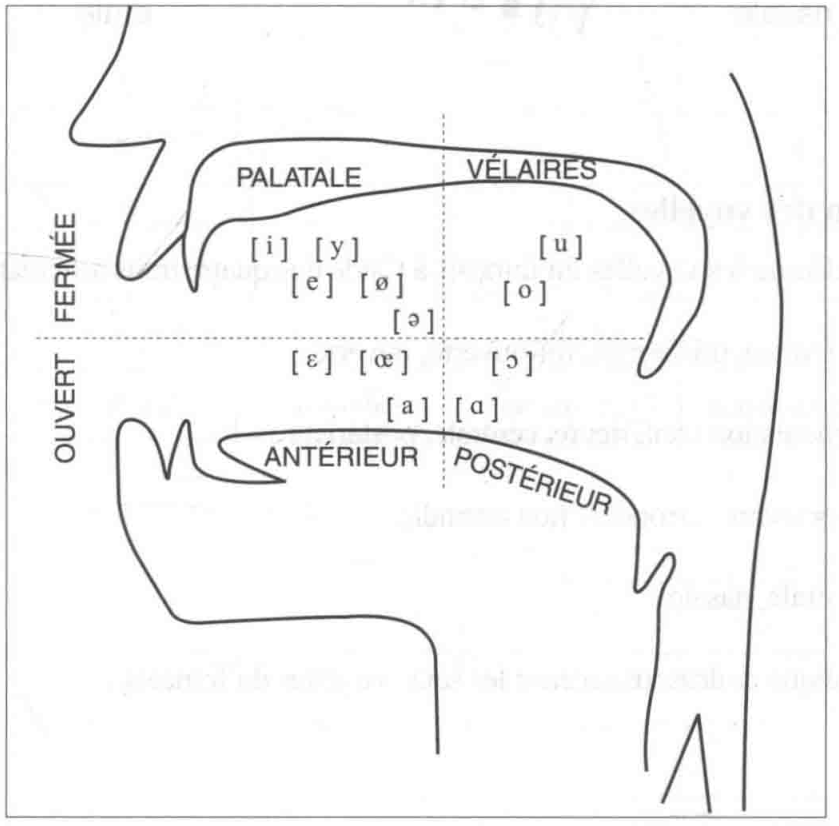
\includegraphics[width=.56\linewidth]{assets/ch07_vowel_positions.png}\end{center}

\origpage{212}{198}
\minititle{\textcircled{\scriptsize 3}\quad Les voyelles arrondies et non arrondies}
Prenons l’exemple des sons \bipa{[i]} de « riz » et \bipa{[y]} de « rue ». Ces deux voyelles sont fermées, et antérieures. Ce qui les distingue est un autre critère important dans la production des voyelles : la labialité. Le \bipa{[y]} de « rue » est produit avec une projection des lèvres vers l’avant, appelée « protrusion », un peu comme lorsqu’on siffle. Les voyelles ainsi produites sont dites arrondies (ou labiales).
\minititle{\textcircled{\scriptsize 4}\quad Les voyelles orales et nasales}
Comme pour les consonnes nasales, la production des voyelles nasales requiert l’ouverture du canal nasal de façon à ajouter une résonance toute particulière à cette voyelle. Si le canal nasal est fermé par la luette, la voyelle sera alors décrite comme orale, comme ci-dessous :
\begin{center}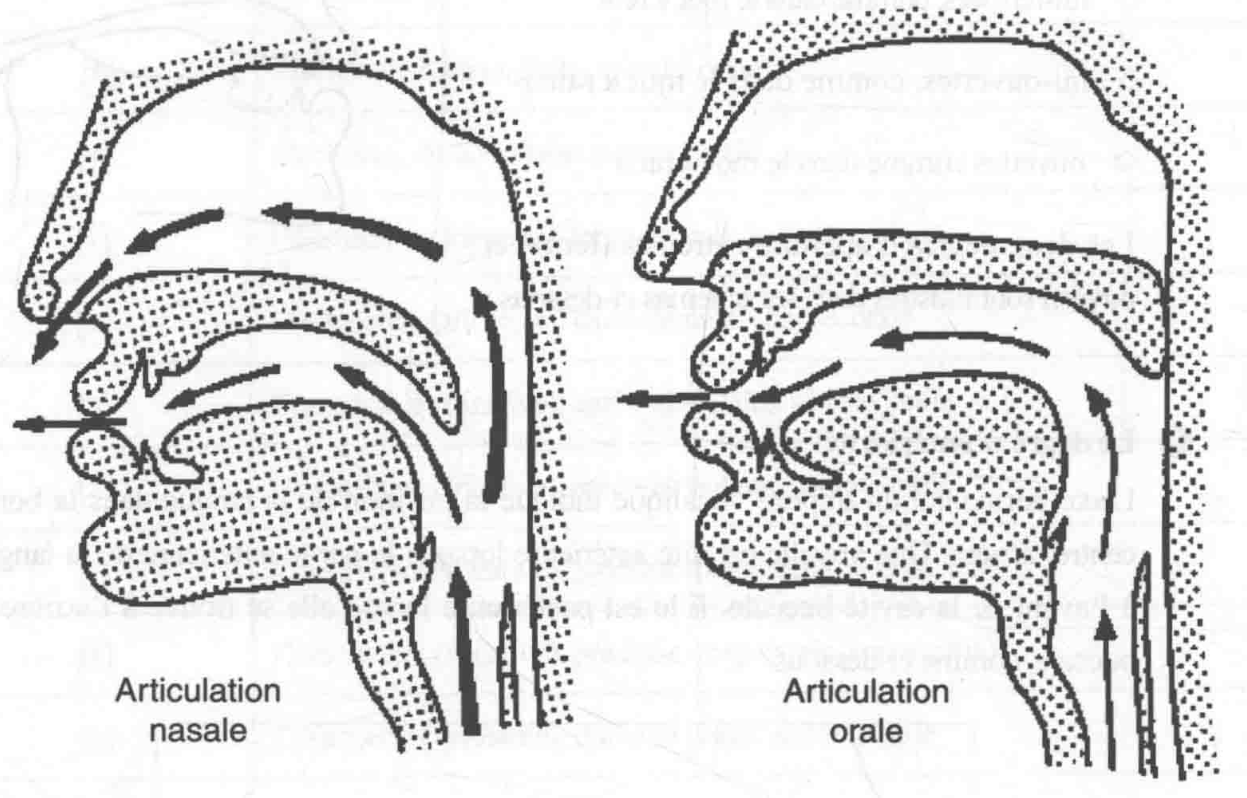
\includegraphics[width=.75\linewidth]{assets/ch07_nasal_oral.png}\end{center}
\subsection{Classification des voyelles}
Nous pouvons décrire les voyelles du français à l’aide des quatre traits articulatoires suivants :
\begin{itemize}
\item l’aperture : fermée, mi-fermée, mi-ouverte, ouverte
\item la zone d’articulation : antérieure, centrale, postérieure
\item la formes des lèvres : arrondie / non arrondie\ednote{原文 la formes 如此；应为 la forme。}
\item la nasalité : orale, nasale
\end{itemize}
Le trapèze vocalique ci-dessous recense les seize voyelles du français :

\origpage{213}{199}
\begin{center}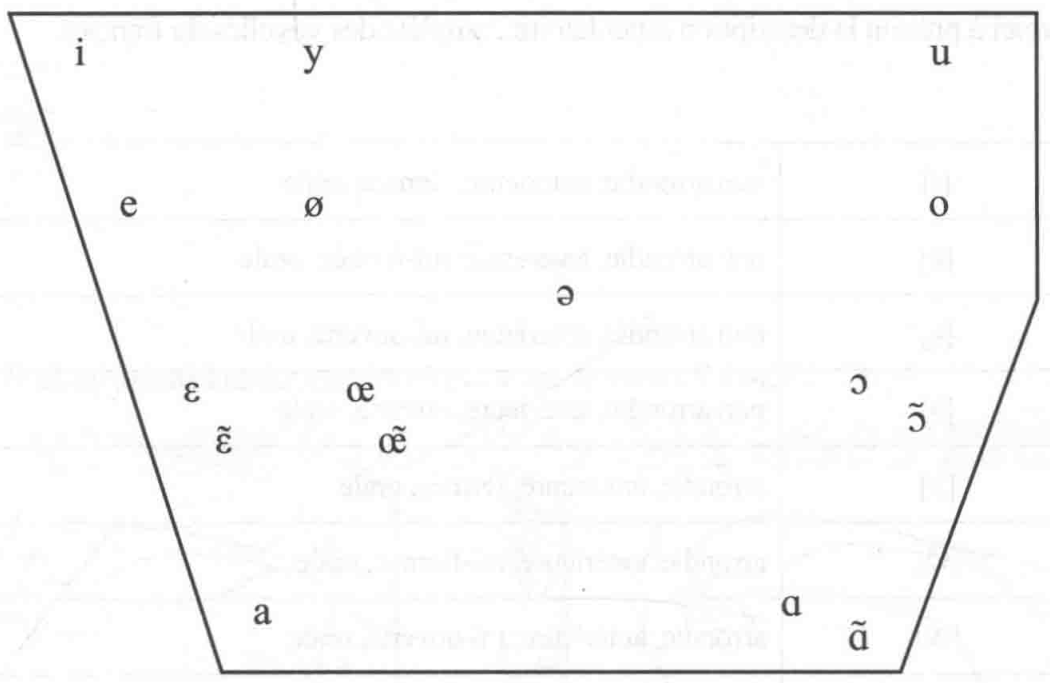
\includegraphics[width=.72\linewidth]{assets/ch07_trapezoid.png}\end{center}
\subsection{Tableaux récapitulatifs}
Il est aussi possible de représenter les voyelles orales et nasales du français sous forme de tableaux en utilisant les descripteurs qui servent à caractériser leur production :
\begin{center}\small\setlength{\tabcolsep}{3pt}\renewcommand{\arraystretch}{1.28}
\begin{tabularx}{\linewidth}{|>{\centering\arraybackslash}p{.16\linewidth}|*{5}{>{\centering\arraybackslash}X|}}
\hline
&\multicolumn{5}{c|}{Orales}\\\cline{2-6}
&\multicolumn{2}{c|}{antérieures}&centrales&\multicolumn{2}{c|}{postérieures}\\\cline{2-6}
&non arrondies&arrondies&non arrondies&non arrondies&arrondies\\\hline
fermées&\bipa{i}&\bipa{y}&&&\bipa{u}\\\hline
mi-fermées&\bipa{e}&\bipa{ø}&&&\bipa{o}\\\hline
moyenne&&&\bipa{ə}&&\\\hline
mi-ouvertes&\bipa{ɛ}&\bipa{œ}&&&\bipa{ɔ}\\\hline
ouvertes&\bipa{a}&&&\bipa{ɑ}&\\\hline
\end{tabularx}
\end{center}
\begingroup\renewcommand{\thefootnote}{校\arabic{editorialnote}}
\begin{center}\small\setlength{\tabcolsep}{3pt}\renewcommand{\arraystretch}{1.28}
\begin{tabularx}{\linewidth}{|>{\centering\arraybackslash}p{.16\linewidth}|*{5}{>{\centering\arraybackslash}X|}}
\hline
&\multicolumn{5}{c|}{Nasales}\\\cline{2-6}
&\multicolumn{2}{c|}{antérieures}&centrales&\multicolumn{2}{c|}{postérieures}\\\cline{2-6}
&non arrondies&arrondies&non arrondies&non arrondies&arrondies\\\hline
fermées&&&&&\\\hline
mi-fermées&&&&&\\\hline
moyenne&&&&&\\\hline
mi-ouvertes&\bipa{ɛ}\ednote{原表 Nasales 中前、不圆唇、半开这一格印为无鼻化符号的 \bipa{ɛ}；据本页元音梯形图及下一页完整分类表，应为 \bipa{ɛ̃}。此处保留原格字形，订正在注中列明。}&\bipa{œ̃}&&&\bipa{ɔ̃}\\\hline
ouvertes&&&&\bipa{ɑ̃}&\\\hline
\end{tabularx}
\end{center}
\endgroup

\origpage{214}{200}
Et voici à présent la description articulatoire complète des voyelles du français.
\begingroup\renewcommand{\thefootnote}{校\arabic{editorialnote}}\small\renewcommand{\arraystretch}{1.2}
\begin{longtable}{|>{\centering\arraybackslash}p{.12\linewidth}|p{.79\linewidth}|}
\hline
\bipa{[i]}&non arrondie, antérieure, fermée, orale\\\hline
\bipa{[e]}&non arrondie, antérieure, mi-fermée, orale\\\hline
\bipa{[ɛ]}&non arrondie, antérieure, mi-ouverte, orale\\\hline
\bipa{[a]}&non arrondie, antérieure, ouverte, orale\\\hline
\bipa{[y]}&arrondie, antérieure, fermée, orale\\\hline
\bipa{[Ø]}\ednote{此格原文用大写 Ø。国际音标的前圆唇半闭元音符号为小写 \bipa{ø}，亦与上页梯形图和口元音表一致。见\ecite{41}。}&arrondie, antérieure, mi-fermée, orale\\\hline
\bipa{[œ]}&arrondie, antérieure, mi-ouverte, orale\\\hline
\bipa{[ə]}&centrale, moyenne\\\hline
\bipa{[u]}&arrondie, postérieure, fermée, orale\\\hline
\bipa{[o]}&arrondie, postérieure, mi-fermée, orale\\\hline
\bipa{[ɔ]}&arrondie, postérieure, mi-ouverte, orale\\\hline
\bipa{[ɑ]}&non arrondie, ouverte, postérieure\\\hline
\bipa{[ɛ̃]}&non arrondie, antérieure, mi-ouverte, nasale\\\hline
\bipa{[ɑ̃]}&non arrondie, postérieure, ouverte, nasale\\\hline
\bipa{[œ̃]}&arrondie, antérieure, mi-ouverte, nasale\\\hline
\bipa{[ɔ̃]}&arrondie, postérieure, mi-ouverte, nasale\\\hline
\end{longtable}\endgroup

Pour terminer, voici le tableau des semi-consonnes du français :\ednote{此表三项均称 constrictive，而前文又把 constrictive 等同 fricative。国际音标中 \bipa{[j]}、\bipa{[ɥ]}、\bipa{[w]} 为近音：分别为硬腭、唇硬腭、唇软腭近音，不应据此表误作带摩擦噪声的擦音。见\ecite{41}。}
\begin{center}\small\renewcommand{\arraystretch}{1.25}
\begin{tabularx}{\linewidth}{|>{\centering\arraybackslash}p{.12\linewidth}|>{\centering\arraybackslash}X|}
\hline
\bipa{[j]}&constrictive, dorso-palatale, sonore, orale, non arrondie\\\hline
\bipa{[ɥ]}&constrictive, dorso-palatale, sonore, orale, arrondie\\\hline
\bipa{[w]}&constrictive, dorso-vélaire, sonore, orale, arrondie\\\hline
\end{tabularx}
\end{center}

Dans le chapitre suivant, nous allons continuer à nous intéresser aux phones, mais du point de vue fonctionnel cette fois-ci : il s’agit des phonème.\ednote{原文 des phonème 如此；应为 des phonèmes。}

\clearpage
\origpage{215}{201}
\section*{Exercices}
\phantomsection\addcontentsline{toc}{section}{Exercices}
\markright{Chapitre 7 — Exercices}
\noindent\textbf{I.\quad Regardez les diagrammes ci-dessous et dites de quel(s) sons il s’agit :}
\begin{center}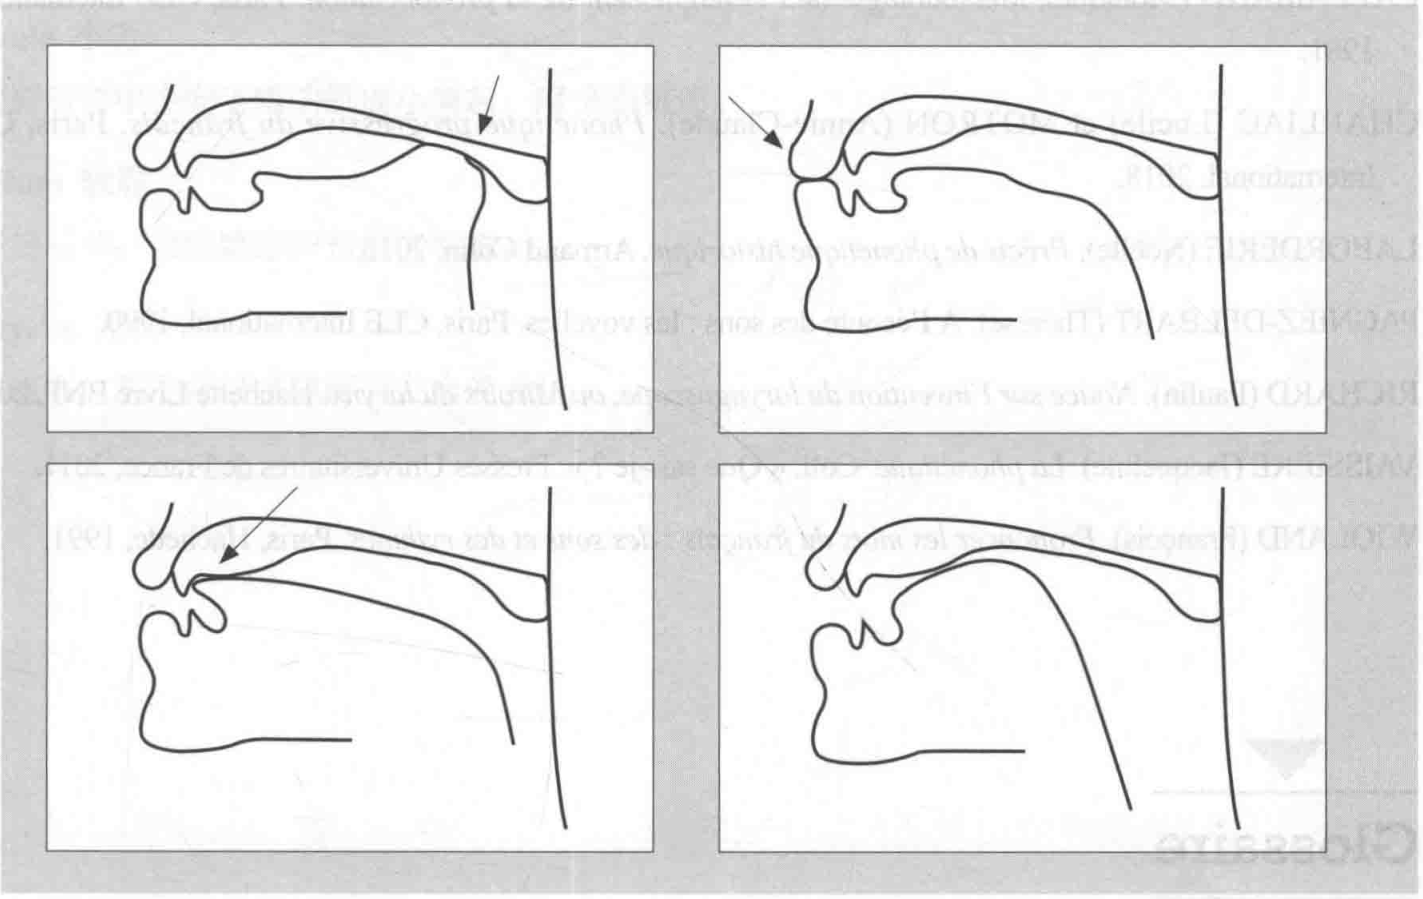
\includegraphics[width=.85\linewidth]{assets/ch07_exercise_diagrams.png}\end{center}
\noindent\textbf{II.\quad Redonnez aux proverbes suivants leur forme originale}
\begin{enumerate}[label=\arabic*.,leftmargin=2em,itemsep=.25em]
\item \bipa{[lepʁɔvɛʁbsɔ̃lelɑ̃pdemo]}
\item \bipa{[lapaʁɔlɛdɑʁʒɑ̃mɛlœsilɑ̃sɛdɔʁ]}
\item \bipa{[lapɛʁlɛsɑ̃valœʁdɑ̃sapʁɔpʁœkɔkij]}
\item \bipa{[labaʁkpas laʁivdœmœʁ]}
\item \bipa{[ʁjɛ̃nœsɛʃplyvitkœlɛlaʁm]}
\item \bipa{[kisɛmlœvɑ̃ʁekɔltlatɑ̃pɛt]}
\item \bipa{[lɔʁskɔ̃tɔ̃b sœnepalœpjekiatɔʁ]}
\item \bipa{[kipesedɛtsɑ̃ʁiʃi]}
\item \bipa{[tʁodœpaʁɔlbuʃlezɔʁɛj]}
\item \bipa{[leʃamonœkipɑɑ̃tʁødœlœʁbɔs]}
\item \bipa{[nylmjɛlsɑ̃fjɛl]}
\item \bipa{[lœʃamɔʁdypaʁœ̃sɛʁpɑ̃ kʁɛ̃mɛmynkɔʁd]}
\end{enumerate}

\origpage{216}{202}
\section*{Pour aller plus loin}
\phantomsection\addcontentsline{toc}{section}{Pour aller plus loin}
\markright{Chapitre 7 — Pour aller plus loin}
\begin{small}
\setlength{\parindent}{0pt}\setlength{\parskip}{.55em}
ABRY (Dominique). \textit{500 exercices de phonétique}. Hachette, 2009.

CALLAMAND (Monique). \textit{Méthodologie de l’enseignement de la prononciation}. Paris, CLE International, 1981.

CHARLIAC (Lucile) et MOTRON (Annie-Claude). \textit{Phonétique progressive du français}. Paris, CLE International, 2018.

LABORDERIE (Noëlle). \textit{Précis de phonétique historique}. Armand Colin, 2015.

PAGNIEZ-DELBART (Thérèse). À l’écoute des sons : les voyelles. Paris, CLE International, 1990.

RICHARD (Paulin). \textit{Notice sur l’invention du laryngoscope, ou Miroirs du larynx}. Hachette Livre BNF, 2013.

VAISSIÈRE (Jacqueline). \textit{La phonétique}. Coll. « Que sais-je ? ». Presses Universitaires de France, 2011.

WIOLAND (François). \textit{Prononcer les mots du français : des sons et des rythmes}. Paris, Hachette, 1991.
\end{small}
\section*{Glossaire}
\phantomsection\addcontentsline{toc}{section}{Glossaire}
\markright{Chapitre 7 — Glossaire}
\gloss{appareil phonatoire 发声器官}{用于发音的口、鼻、喉的某一部位。\ednote{“某一部位”范围不当；appareil phonatoire 指参与发声的器官系统，不是口、鼻、喉中某个单一部位。本章正文还明确列入肺、气管及相应肌肉。}}
\gloss{consonne 辅音}{发音时气流通路受阻碍的音。}
\gloss{cordes vocales 声带}{从喉的后部延伸到前部的坚韧、柔软的组织。}
\gloss{fricative 擦音}{辅音的一种，因出口狭窄，空气流出时产生明显的摩擦。}
\gloss{larynx 喉}{气管（喉中）上部由软骨和肌肉组成的一段管子，内有声带。\ednote{“气管（喉中）”混淆喉与气管的位置及包含关系。喉是连接咽与气管、位于气管上方的独立结构，内含声带；不能说气管处于喉内。见\ecite{43}，Larynx 与 Trachea 两节。}}

\origpage{217}{203}
\gloss{nasale 鼻音}{辅音的一种，气流在口腔受阻塞但允许通过鼻腔发出。}
\gloss{palais dur 硬腭}{腭的前部，由骨和肌肉构成。\ednote{硬腭的支架为骨，表面覆以黏膜等软组织；不能把其结构与主要由肌肉构成的软腭混同。“由骨和肌肉构成”宜订正为“以骨为支架、表面覆有黏膜的腭前部”。见\ecite{42}。}}
\gloss{pharynx 咽}{喉咙中声带至口腔后部软腭之间的部分。发音时，其形状和容积可通过各种方式加以改变。\ednote{此释义只近似描述语音学中的一段咽腔，不能作为完整解剖定义：咽分鼻咽、口咽、喉咽，声带位于喉内，不是整个咽的边界。见\ecite{42}、\ecite{43}。}}
\gloss{uvule 小舌}{软腭后部中央向下垂的肌肉小突起，略呈圆锥形。}
\gloss{vélum 软腭}{腭的后部，由结缔组织和肌肉构成。}
\gloss{voyelle 元音}{气流在口腔不受显著阻碍而发出的音。}
